% This is samplepaper.tex, a sample chapter demonstrating the
% LLNCS macro package for Springer Computer Science proceedings;
% Version 2.20 of 2017/10/04
%
\documentclass[runningheads]{llncs}
%
\usepackage{xcolor}
\usepackage{graphicx}
\usepackage{makecell}
\usepackage{textcomp}
%\usepackage{amsmath,amssymb,amsfonts}
\usepackage{algorithm,algorithmic}
% Used for displaying a sample figure. If possible, figure files should
% be included in EPS format.
%
% If you use the hyperref package, please uncomment the following line
% to display URLs in blue roman font according to Springer's eBook style:
% \renewcommand\UrlFont{\color{blue}\rmfamily}

\renewcommand{\baselinestretch}{0.97}

\begin{document}
%
%\title{Automated Formal Synthesis of Optimal Sizing for Stand-alone Solar Photovoltaic Systems\thanks{Supported by Newton Fund (ref. 261881580) and FAPEAM (Amazonas State Foundation for Research Support, calls 009/2017 and PROTI Pesquisa 2018).}}
\title{Synthesis of Solar Photovoltaic Systems: Optimal Sizing Comparative\thanks{Supported by Newton Fund (ref. 261881580) and FAPEAM (Amazonas State Foundation for Research Support, calls 009/2017 and PROTI Pesquisa 2018).}}
%
%\titlerunning{Abbreviated paper title}
% If the paper title is too long for the running head, you can set
% an abbreviated paper title here
%
\author{Alessandro Trindade\inst{1}\orcidID{0000-0001-8262-2919} \and
Lucas Cordeiro\inst{2}\orcidID{0000-0002-6235-4272}}
%
\authorrunning{A. Trindade and L. Cordeiro}
% First names are abbreviated in the running head.
% If there are more than two authors, 'et al.' is used.
%
\institute{Federal University of Amazonas, Av. Gen. Rodrigo Octavio, 6200, Coroado I, 69077-000 Manaus AM Brazil \email{alessandrotrindade@ufam.edu.br} \and
The University of Manchester, Kilburn Building, Oxford Road, Manchester M13 UK
\email{lucas.cordeiro@manchester.ac.uk}}
\maketitle              % typeset the header of the contribution

\begin{abstract}
%Currently, there exist various state-of-the-art tools to design solar photovoltaic (PV) systems, but they are mainly based on simulations, which do not cover all aspects of the design-space. We present a sound and automated approach to synthesize optimal sizing of stand-alone PV systems using program synthesis. In particular, our variant of counterexample guided inductive synthesis (CEGIS) approach has two phases: first we synthesize sizing of stand-alone PV systems but that may not achieve the lowest cost. The optimal solution is then verified via symbolic model checking; if the verification step fails, a counterexample is provided to the synthesis engine and the process iterates until an optimal sizing is obtained. Commercial equipment data is provided to our synthesis engine and candidate solutions are derived from financial analysis of the obtained sizing. Our synthesis method is novel and unprecedented to streamline the design of PV systems. Experimental results show that our synthesis method is able to synthesize within an acceptable run-time the optimal PV system sizing of seven different intricate case studies.
In 2017, for the first time, the number of people without access to electricity dipped below 1 billion, but trends in energy access still fall short of global goals. Particular attention is given to stand-alone solar photovoltaic systems in rural areas or where grid extension is unfeasible. Tools to evaluate or to size electrification projects are available, but they are based on simulations that do not cover all aspects of the design space. The use of formal methods in electrical systems is a new subject, with published research spanning only the last four years. Moreover, the use of automated synthesis in order to obtain optimal sizing of solar photovoltaic systems has never been done before; this is our major goal: a sound, automated approach to obtaining optimal sizing of stand-alone photovoltaic systems using program synthesis. We propose a variant of the counterexample guided inductive synthesis (CEGIS) approach, with two phases linking the technical and the cost analysis. First, we synthesize a feasible candidate based on power reliability, but which may not attain the lowest cost. Second, the candidate is then verified iteratively with a lower bound cost via symbolic model checking. If the verification step succeeds, the lower bound is adjusted; if it fails, a counterexample provides the optimal solution. Experimental results using seven case studies demonstrate that we can produce optimal solution within an acceptable run-time. We also present a comparison with a specialized simulation tool over real photovoltaic systems in order to show the effectiveness of our approach.
\keywords{Automated verification  \and Model Checking \and Electric systems \and Solar photovoltaic systems.}
\end{abstract}
%

%%%%%%%%%%%%%%%%%%%%%%%%%%%%%%%%%%%%%%%%%%%%%%%%%%%%%%%%
\section{Introduction}
%%%%%%%%%%%%%%%%%%%%%%%%%%%%%%%%%%%%%%%%%%%%%%%%%%%%%%%%

Cyber-Physical Systems  (CPS) are engineered systems, which are built from, and depend upon, 
the seamless integration of computational  and  physical  components~\cite{NSF2015}. 
During operation, such components must frequently adapt to the executing environment changes 
faced at run-time (dynamics of the physical processes) and must be able to continue to behave 
in a controlled and safe way, thus posing novel technical challenges for the software engineering of services and applications for CPS~\cite{Metzger2014}. %Important quality aspects for CPS include scalability, e.g., ensuring that CPS applications can scale to urban-wide deployment environments [Nessi].
%Software pervasiveness in CPS places new challenges; in particular, highly dynamic environments, rapidly changing requirements, 
%unpredictable and uncertain operating conditions demand new paradigms for software design~\cite{Filieri2015}.
%
%While some research efforts do exist to enhance and optimize the software development processes for CPS, further investigation and discussion of better and more effective models are still needed in practice~\cite{Al-Jaroodi2016}. 
Among the opportunities for enhancements in the software development processes for CPS, there exists the need for developing new techniques and tools to support CPS requirements gathering and analysis with the goal of synthesizing correct-by-construction implementations of CPS. These techniques need to deal with predefined requirements enforced by the nature and inherited constraints of the target CPS. In addition, they should be able to provide verification and validation mechanisms for completeness, correctness, and consistency~\cite{Al-Jaroodi2016}. Uncertainty and variability, at the same time, can be dealt with formal verification~\cite{NESSI}. Energy production, distribution, and optimization are all CPS problems~\cite{UC}. 

Lack of access to clean and affordable energy is considered a core dimension of poverty~\cite{Hussein2012}. Progress has been made worldwide; in particular, the number of people without electricity access fell below $1$ billion threshold for the first time in 2017~\cite{IEAweo2018}. To provide universal electricity for all, decentralized systems led by solar photovoltaic (PV) in off-grid and mini-grid systems will be the lowest-cost solution for three-quarters of the additional connections needed~\cite{Hussein2012}; specifically grid extension will be the standard in urban areas~\cite{IEAweo2018}.

In order to simulate or evaluate a PV system, there exist various specialized tools, e.g., RETScreen and HOMER~\cite{Pradhan,Swarnkar}%, PVWatts, SAM and Hybrid2 \cite{Pradhan,Swarnkar,NRELDobos,NRELBlair,Mills}
; and even general purpose simulation tools, e.g., MATLAB/Simulink~\cite{Gow1999}. %PSpice, Saber or MATLAB/Simulink package \cite{Gow1999,Benatiallah2017}.
 However, these tools are based on simulation; they have the drawback of an incomplete coverage  since verification of all possible combinations and potential failures of a system is unfeasible~\cite{ClarkeHV18}. 
 Optimization of PV systems is not a recent topic; since the 90's different techniques using different criteria to find ultimate combinations for design parameters, based on intuitive, numerical and analytical methods were proposed and developed~\cite{Alsadi2018}.
 
However, formal methods based on \textit{symbolic model checking} and its application to synthesize PV systems have not been further explored, which can offer a great potential to obtain a more effective design process to PV systems~\cite{ClarkeHV18}. Here, we use counterexample guided inductive synthesis (CEGIS) for synthesizing optimal sizing of stand-alone PV systems using commercial equipment data. Given a correctness specification $\sigma$, our method uses that as starting point and then iteratively produces a sequence of candidate solutions that satisfy $\sigma$. In particular, in each iteration, we synthesize sizing of stand-alone PV systems but that may not achieve the lowest cost. The optimal solution is then verified via symbolic model checking; if the verification step fails, a counterexample is provided to the synthesis engine and the process iterates until an optimal sizing is obtained from financial analysis.

Related to past work, in $2012$, a Chinese smart grid implementation considered a case study to address the verification problem for performance and energy consumption~\cite{Yukseletall2012}. In $2015$, an automated simulation-based verification technique was applied to verify the correctness of power system protection settings~\cite{Sengupta2015}. In $2017$, a researcher suggested the application of formal methods to verify and control the behavior of computational devices in a smart grid ~\cite{Abate2017}. Finally, in $2018$, a verification methodology was applied to PV panels and its distributed power point tracking~\cite{Driouich2018}. However, prior studies did not deal with electricity generation or even solar PV systems optimization. Formal methods based on \textit{symbolic model checking} and its application to synthesize PV systems are still unexplored in literature.

Our work makes two major contributions. Firstly, the use of automated symbolic verification in electrical systems was uncommon in recent prior studies~\cite{TrindadeCordeiro19}, and specifically their use in synthesizing PV sizing is unprecedented. Here, a list of PV components %(i.e., PV panels, charge controllers, inverters, and batteries) 
can be fed to our proposed synthesis method together with user requirements and environment constraints, and our synthesis algorithm based on symbolic model checking can find the optimal solution in technical and economical terms. Secondly, we evaluate different state-of-art symbolic software verifiers with the goal of obtaining the best performance in our verification back-end for synthesizing optimal PV systems.

%-----------------------------------------------------------
\section{BACKGROUND}
\label{sec:AutomatedVerification}
%-----------------------------------------------------------
%
%-----------------------------------------------------------
\subsection{Program Synthesis}
\label{sec:ProgramSynthesis}
%-----------------------------------------------------------
%
The basic idea of program synthesis is to automatically construct a program $P$ that satisfies a correctness specification $\sigma$. In particular, program synthesis is automatically performed by engines that use a correctness specification $\sigma$, as starting point, and then incrementally produce a sequence of candidate solutions that partially satisfy $\sigma$~\cite{Abateetal2017}. As a result, a given candidate program $p$ is iteratively refined, in order to match $\sigma$ more closely. CEGIS represents one of the most popular approaches to program synthesis that are currently used in practice for CPS~\cite{Abateetal2017}, whose basic architecture is illustrated in Figure~\ref{Counter-Example-Guided-Inductive-Synthesis} and has close connections to algorithmic debugging using counterexamples and abstraction refinement~\cite{Alur}. 

The correctness specification $\sigma$ provided to our program synthesizer is of the form $\exists \vec{F} .  \forall \vec{x}.  \sigma(\vec{x}, \vec{F})$, where $\vec{F}$ ranges over functions, $\vec{x}$ ranges over ground terms, and $\sigma$ is a quantifier-free (QF) formula typically supported by SMT solvers. The ground terms are interpreted over some finite domain $\mathcal{D}$, where $\mathcal{D}$ can be encoded using the SMT's bit-vectors part. Examples of specification used by our method include house demand, energy, and battery autonomy; we also provide a list of equipment specification and price from different manufacturers and models.

In Figure~\ref{Counter-Example-Guided-Inductive-Synthesis}, the phases {\sc Synthesize} and {\sc Verify} interact via a finite set of test vectors {\sc inputs} that is incrementally updated. Given the correctness specification $\sigma$, the {\sc Synthesize} procedure tries to find an existential witness $\vec{F}$ satisfying the specification $\sigma(\vec{x}, \vec{F})$, for all $\vec{x}$ in {\sc inputs} (as opposed to all $\vec{x} \in \mathcal{D}$). If {\sc synthesize} succeeds in finding a witness~$\vec{F}$, the latter is a candidate solution (i.e., feasible combination of equipment) to the full synthesis formula, which is passed to {\sc verify}, in order to check whether it is a proper solution ({\it i.e.}, $\vec{F}$ satisfies the specification $\sigma(\vec{x}, \vec{F})$ for all $\vec{x}\in\mathcal{D}$). If this is the case, then the algorithm terminates, i.e., we have found a feasible equipment with the lowest cost; otherwise, additional information is provided to the phase {\sc synthesize}, in the form of a new counterexample that is added to the {\sc inputs} set and the loop iterates again. 
%
\begin{figure}[h]
	\centering
	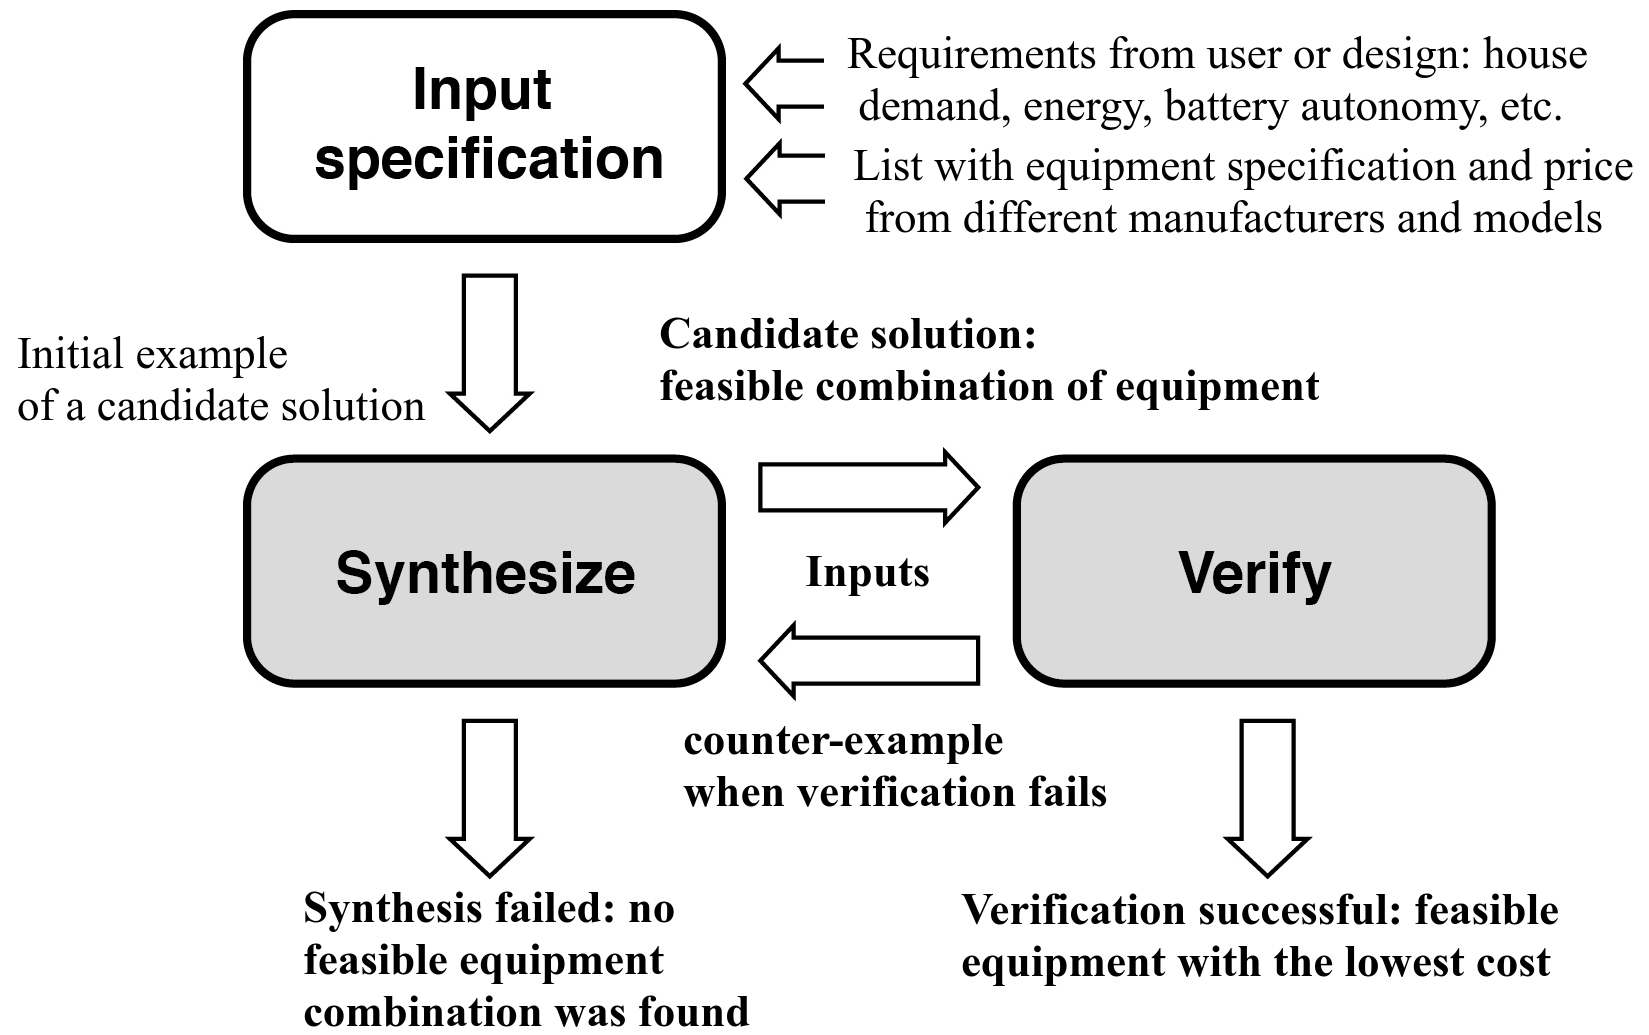
\includegraphics[width=0.85\columnwidth]{fig2_rev.jpg}
	\caption{CEGIS applied to PV system sizing.}
	\label{Counter-Example-Guided-Inductive-Synthesis}
\end{figure}
%
One may notice that each iteration of the CEGIS loop adds a new input to the finite set $INPUTS$, which is then used for synthesis.  Given that the full set of inputs $\mathcal{D}$ is finite because we use bit-vector expressions, this means that the refinement loop can only iterate over a finite number of times; however, {\sc synthesize} may conclude that no candidate solution obeying $\sigma$ for the finite set $INPUTS$ exists and our synthesis engine can then conclude that no feasible equipment combination was found. At this specific automated formal synthesis of PV systems, we use a variant of CEGIS, where in each iteration we increase the expected cost of PV systems and this controls the {\sc verify} phase and the search by the optimal sizing.  %however, $\mathcal{D}$ can represent a large number of elements for the finite set  and our synthesis engine can then conclude that no feasible equipment combination was found. 
%In order to avoid exploring all possible values, machine learning techniques can be used in the phase {\sc synthesize}, with the goal of learning from experience (input-output samples), {\it i.e.}, learning from counterexamples provided by a verification oracle~\cite{Alur13}. In addition to that, a pre-processing stage could also figure as another block in the scheme shown in Fig. \ref{Counter-Example-Guided-Inductive-Synthesis}, between {\sc verify} and {\sc synthesize}, which would process counterexamples and provide larger and refined information to the latter, according to specification $\sigma$ and domain $\mathcal{D}$, in order to speed-up convergence to a final candidate.
Program synthesis engines that implement the CEGIS approach~\cite{sketch} can automatically produce solutions for a large variety of specifications, due to the combination of automated testing, genetic algorithms, and SMT-based reasoning~\cite{Sharma14}; here we have used software verifiers based on SMT solvers: %Here we used software model checking techniques implemented by different tools: 
CPAChecker~\cite{Beyer2011}, CBMC~\cite{Kroening}, and ESBMC~\cite{esbmc2018}.

\textbf{CPAchecker}~\cite{LMU2019} is a state-of-the-art model checker, awarded with the golden medal at the annual competition in software verification: Automatic program verification requires a choice between precision and efficiency. The more precise a method, the fewer false positives it produces, but also the more expensive it is, and thus applicable to fewer programs. Historically, this trade-off was reflected in two major approaches to static verification: program analysis and model checking. To experiment with the trade-off and to be able to set the dial between the two extreme points, Configurable Program Analysis (CPA) provides a conceptual basis for expressing different verification approaches in the same formal setting. The CPA formalism provides an interface for the definition of program analysis. Consequently, CPAchecker provides an implementation framework that allows the seamless integration of program analysis expressed in the CPA framework. In terms of the architecture, the central data structure is a set of control-flow automata (CFA), which consists of control-flow locations and control-flow edges. The CPA framework provides interfaces to SMT (Satisfiability Modulo Theories) solvers and interpolation procedures~\cite{Beyer2011}. Currently, CPAchecker uses MathSAT as SMT solver~\cite{Beyer2011}.

The C Bounded Model Checker (\textbf{CBMC}) falsifies assertions in C programs or proves that they are safe if a completeness threshold is given~\cite{Kroening}. CBMC implements a bit-precise translation of a C program, annotated with assertions and with loops unrolled up to a given depth, into a logical formula. If the formula is satisfiable, then a failing execution that leads to a violated assertion exists~\cite{Kroening}. CBMC's verification flow can be summarized in three stages: (i) Front-end: scans, parses and type-checks C code; it converts control flow elements, such as \textit{if} or \textit{switch} statements, loops and jumps, into equivalent guarded \textit{goto} statements, thus aiming to reduce verification effort; (ii) Middle-end: performs symbolic execution by eagerly unwinding loops up to a fixed bound, which can be specified by the user on a per-loop basis or globally, for all loops and finally; (iv) Back-end: supports SAT and SMT solvers to discharge verification conditions.

The Efficient SMT-based Bounded Model Checker (\textbf{ESBMC}) is a bounded and unbounded model checker for C programs~\cite{esbmc2018}, which supports the verification of LTL properties with bounded traces~\cite{DBLP:journals/sosym/MorseCN015}. ESBMC's verification flow can be summarized in three stages: (i) a front-end that can read and compile C code, where the system formal specification is first handled; (ii) preprocessing steps to deal with code representation, control flow and unwinding of loops, and model simplification, thereby aiming to reduce verification effort; and finally (iii) the SMT solving stage, where all constraints and properties of the system are encoded into SMT and checked for satisfiability. ESBMC exploits the standardized input language of SMT solvers (SMT-LIB\footnote{http://smtlib.cs.uiowa.edu/} logic format) to make use of a resource called \textit{assertion stack}~\cite{Morse2015}. This enables ESBMC, and the respective solver, to learn from previous checks, thus optimizing the search procedure and potentially eliminating a large amount of formula state space to be searched, because it solves and disregards data during the process, incrementally. This technique is called ``incremental SMT''~\cite{DBLP:journals/fac/SchrammelKBMTB17} and allows ESBMC to reduce the memory overhead, mainly when the verified system is complex and the computing platform does not have large amount of memory to deal with the entire design space state.

%%%%%%%%%%%%%%%%%%%%%%%%%%%%%%%%%%%%%%%%%%%%%%%%%%%%%%%%
\subsection{Sizing Stand-alone Solar PV Systems}
\label{sec:sizing}
%%%%%%%%%%%%%%%%%%%%%%%%%%%%%%%%%%%%%%%%%%%%%%%%%%%%%%%%
A PV system is illustrated in Fig.\ref{fig:blockdiagram}. %It identifies the PV generator, batteries, charge controller, inverter, and AC load. 
The PV generator, which can be a panel or an array, is a semiconductor device that can convert solar energy into DC electricity. %In Fig.\ref{fig:blockdiagram}, there are two variables that depend on the site where the system is deployed and also the weather (i.e., solar irradiance $G$ and temperature $T$). 
For night hours or rainy days, we hold batteries where power can be stored and used. The use of batteries as a storage form implies the presence of a charge controller~\cite{Hansen}. The PV arrays produce DC and therefore when the PV system contains an AC load, a DC/AC conversion is required. That converter is called inverter; and the AC load dictates the behavior of AC electrical load from the house that will be fed by the system.
\begin{figure}[h]
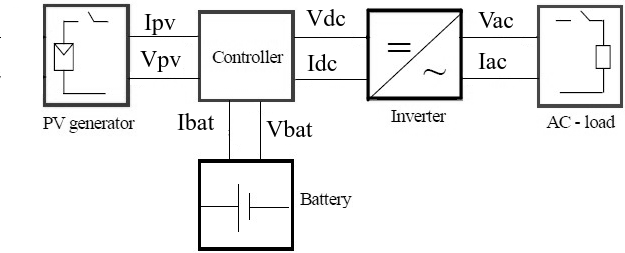
\includegraphics[width=0.4\textwidth]{blockdiagramPVS2_rev}
\centering
\caption{Block diagram for a typical stand-alone PV system~\cite{Hansen}.}
\label{fig:blockdiagram} 
\end{figure}
\\
%
The sizing check stage will ensure that the system meets the standard project steps related to critical period solar energy method~\cite{Pinho} and adopting MPPT (Maximum Power Point Tracking) charge controller, which is the most common one in practice. 
%
Firstly, we need to correct the energy consumption estimated to the load ($E_{consumption}$), which is carried out by Eq.~\ref{eq:Ecorrected}, where the efficiency of batteries ($\eta_{b}$), controller ($\eta_{c}$), and inverter ($\eta_{i}$) are considered~\cite{Pinho} as follows

\begin{equation}
\label{eq:Ecorrected}
E_{corrected} = \frac {E_{consumption}}{\eta_{b} \eta_{c} \eta_{i} }.
\end{equation}

We also need to estimate the energy that can be produced for each panel, called $E_{p}$, in Wh, defined as

\begin{equation}
\label{eq:Ep}
E_{p} = Solar\_Irradiance \times Panel\_Area \times \eta_{p} \times 1000,
\end{equation}

\noindent where the solar irradiance is expressed in terms of $kWh/m^{2}$ and depends on the site where the PV system will be deployed; 
the PV panel area is given in $m^{2}$ and corresponds to the size of one PV panel, and $\eta_{p}$ represents the PV panel efficiency.
%
The total minimum number of needed solar panels ($N_{TPmin}$) is computed as
%
\begin{equation}
\label{eq:NTPmin}
N_{TPmin} = \frac{E_{corrected}}{E_{p}}.
\end{equation}
%
Particularly, the total number of panels in series ($N_{PSmin}$) and parallel ($N_{PPmin}$) are respectively given by
%
\begin{equation}
\label{eq:NPSmin}
\frac{V_{mppt,min}}{V_{maxPower,TempMax}} \leq N_{PSmin} \leq \frac{V_{mppt,max}}{V_{maxPower,TempMin}},
\end{equation}
%
\begin{equation}
\label{eq:NPPmin}
N_{PPmin} = \frac{P_{total}}{Number\,Panels\,Series \times P_{max,ref}},
\end{equation}
%
\noindent where $V_{mppt,max}$ is the maximum operation voltage and $V_{mppt,min}$ is the minimum operation voltage of the charge controller; $V_{maxPower,TempMax}$ and $V_{maxPower,TempMin}$ are the maximum power voltage from the PV module considering the maximum and minimum operational temperature, respectively; $P_{total}$ is the total power demanded from the PV system and $P_{max,ref}$ is the power supplied from one PV panel in $Watts$.
%, $ V_{system} $ is the DC voltage of the bus, normally $12$, $24$ or $48$ V.
%
Regarding batteries, we must first define the total capacity of the battery bank, which can be described as
\begin{equation}
\label{eq:Cbank}
C_{bank} = \frac{E_{corrected} \times autonomy}{V_{system} \times DOD},
\end{equation}
%
\noindent where the variable $autonomy$ is a design definition; % and normally has a value ranging from $6$ to $48$h; 
$ V_{system} $ is the DC voltage of the bus, and $ DOD $ is the battery deep of discharge (considered of maximum of 25\% here).
%
Secondly, the total (minimum) number of batteries is computed as 
\begin{equation}
\label{eq:Nbtotal}
N_{B}total = N_{BS}min \times N_{BP}min = \frac{V_{system}}{V_{bat}} \times \frac{C_{bank}}{Battery \, Capacity}.
\end{equation}
%
Regarding the charge controller, it must initially meet the voltage requirement of the PV system, as described by Eq.~\ref{eq:vcvsystem} to the charge controller voltage: 
\begin{equation}
\label{eq:vcvsystem}
V_{c} = V_{system}.
\end{equation}
%
The short circuit reference information from the manufacturer's solar panel must be corrected to the cell temperature because the field temperature is higher than the nominal or laboratory temperature, and PV system is temperature dependent, as 
%
\begin{equation}
\label{eq:iscamb}
I_{sc,amb} = \frac{G}{G_{ref}} \left[I_{sc,ref} +  \mu_{I} \times (T-25) \right]. 
\end{equation}
%
The controller must meet the maximum current from the PV array given by Eqs. \ref{eq:icmin} and \ref{eq:icicmin} as
\begin{equation}
\label{eq:icmin}
I_{c,min} = I_{sc,amb} \times N_{PP},
\end{equation}
%
\begin{equation}
\label{eq:icicmin}
I_{c} \geq I_{c,min}.
\end{equation}
%
The inverter sizing check is performed by means of three equations. Eq.~\ref{eq:vindc} ensures that the input voltage of the controller meets the system voltage. Eq.~\ref{eq:voutac} ensures that the output voltage of the controller meets the AC voltage of the load. Finally, Eq.~\ref{eq:invcheck} ensures that the controller can support the total demand of the load ($Demand$) and the surge power ($P_{surge}$), where $V_{in}DC$ is the nominal input voltage and $V_{out}AC$ is the nominal output voltage of the inverter; $MAX_{AC,ref}$ is the peak power that the inverter can support.
%
\begin{equation}
\label{eq:vindc} 
V_{in}DC = V_{system}.
\end{equation}
%
\begin{equation}
\label{eq:voutac} 
V_{out}AC = V_{AC}.
\end{equation}
%
\begin{equation}
\label{eq:invcheck} 
\left[ (Demand \leq P_{AC,ref}) \, and \, (P_{surge} \leq MAX_{AC,ref}) \right].
\end{equation}
% -------------------------------------------------------
\subsection{Optimal Sizing of PV Systems}
% -------------------------------------------------------
%
%%%To select an optimal combination of components from a PV system to meet sizing constraints, 
%we need to evaluate \textit{power reliability} and perform \textit{system cost} analysis for the recommended system. An ideal combination for any PV system 
The optimal sizing of PV systems is made by the best compromise between two objectives: power reliability and system cost~\cite{Alsadi2018}. 
Regarding power reliability, this work will rely on the critical period solar energy method~\cite{Pinho} as described in section~\ref{sec:sizing}. 
%the usual is to use loss of load probability (LOLP) or loss of power supply probability (LPSP). Based on the fact that here we are neither considering site characteristics nor the load changes over time, the reliability analysis will be developed only by the critical period method of PV sizing \textcolor{red}{What does it mean? Remember that we have software engineering audience}. 
%However, considering the system cost analysis, we usually find related studies done with Net Present Cost (NPC), Levelized Cost of Energy (LCOE), or Life Cycle Cost (LCC). Here, based on the fact that the deployment location is not specified, our study uses an adapted LCC analysis, where only the deployment cost is considered about the model, i.e., without the operational and maintenance costs~\cite{Alsadi2018}.
Considering the system cost analysis, based on the fact that the deployment location is not specified, our study uses an adapted Life Cycle Cost (LCC) analysis, where only the acquisition cost is considered about the model, i.e., without the operational and maintenance costs~\cite{Alsadi2018}.
%------------------------------------------------------
\section{Synthesizing Optimal Sizing of Stand-alone Solar Photovoltaic Systems}
%Applying Automated Verification to Optimal Sizing of Stand-alone Solar PV Systems}
%------------------------------------------------------
Algorithm~\ref{alg:verification-algorithm} describes our pseudo-code to synthesize stand-alone PV systems using symbolic model checking. 
%
 \begin{algorithm}
 \caption{Synthesis algorithm}
 \begin{algorithmic}[1]
 \begin{scriptsize}
 \renewcommand{\algorithmicrequire}{\textbf{Input:}}
 \renewcommand{\algorithmicensure}{\textbf{Output:}}
  \STATE Initialize variables \\
  \STATE Declare list of PV panels, controllers, batteries, and inverters data and cost \\
%  \STATE Declare list of controllers data and cost \\
%  \STATE Declare list of batteries data and cost \\
%  \STATE Declare list of inverters data and cost \\
  \STATE Declare the maximum possible cost $MaxCost$  \\
  \STATE Declare power demand, power peak, energy consumption \\
  \STATE Declare battery autonomy, deep of discharge, AC voltage \\
  \FOR {$HintCost=0$ to $MaxCost$}
 	\STATE Declare non-deterministic variable to select PV Panel from list \\
 	\STATE Declare non-deterministic variable to select Controller from list \\
 	\STATE Declare non-deterministic variable to select Battery from list \\
 	\STATE Declare non-deterministic variable to select Inverter from list \\ 	
 	\STATE Calculate $E_{corrected}, \, E_{p} $ \\
	\STATE Calculate $N_{TPmin}, \, N_{PSmin}, N_{PPmin} $ \\
 	\STATE Calculate $C_{bank}$ \\
	\STATE Calculate $N_{BS}min, \, N_{BP}min, \, N_{B}total$ \\
	\STATE Requirement enforced by \textbf{assume}$(V_{c})$ \\
 	\STATE Calculate $I_{sc,amb}$ \\
 	\STATE Calculate $I_{c,min}$ \\
 	\STATE Requirement enforced by \textbf{assume}$(I_{c} \wedge V_{in}DC \wedge V_{out}AC)$ \\
%	\STATE Requirement enforced by \textbf{assume}$(V_{in}DC \wedge V_{out}AC )$ \\
%	\STATE Requirement enforced by \textbf{assume}$(V_{out}AC)$ \\
	\STATE Requirement enforced by \textbf{assume}$(Demand \wedge P_{surge})$ \\
%	\STATE Requirement enforced by \textbf{assume}$(P_{surge})$ \\
	\STATE non-deterministic variables hold feasible equipment and cost  \\
	\STATE $F_{obj} \leftarrow  N_{TP}*Panel_{Cost} \, + \, N_{TB}*Battery_{Cost} \, + Controller_{Cost} \, + \, Inverter_{Cost}$ \\
	\STATE Violation check with \textbf{assert}$(F_{obj} > HintCost)$ \\
  \ENDFOR
 \RETURN $(\,)$ 
  \end{scriptsize}
 \end{algorithmic} 
 \label{alg:verification-algorithm}
 \end{algorithm}
%

Our synthesis algorithm will synthesize constant values; it starts with the input of manufacturers data and prices of PV panels, batteries, charge controllers and inverters (Line 2). After that, we define user requirements, i.e., house requirements and design definitions, from Lines 4 and 5. 

The \textit{for}-loop started at Line 6 controls the lowest cost to the PV solution. In particular, it starts with cost $0$ and stops only when the algorithm finds a feasible solution in which the cost breaks the $assertion$ stated in Line 22; if that happens, then our algorithm has found an optimal solution, thereby stating that the {\sc Verify} phase reached a satisfiable condition (\textit{SAT}). The $MaxCost$ value at Line 6 is just a very high value put as a limit to the \textit{for}-loop, that never will be reached because the optimal solution will be found first.

Our synthesis algorithm uses non-deterministic variables to choose one specific constant from a given list of PV panels, controllers, batteries and inverters (Lines 7 to 10). That procedure ensures that our synthesis engine checks all combinations of items from each equipment, and combine them to assemble a feasible (candidate) PV solution, which meets the user requirements.

Next, we use Eq.~\ref{eq:Ecorrected}, Eq.~\ref{eq:Ep}, Eq.~\ref{eq:NTPmin}, Eq.~\ref{eq:NPSmin}, Eq.~\ref{eq:NPPmin}, Eq.~\ref{eq:Cbank}, Eq.~\ref{eq:Nbtotal}, Eq.~\ref{eq:iscamb}, and Eq.~\ref{eq:icmin} to calculate the sizing variables (Lines 11 to 17). The directive \textit{assume} (Lines 15, 18 and 19) ensures the compatibility of the chosen items from the list of equipment: the {\sc Verify} phase uses only the item (among all the possible ones) that satisfies the statements of Lines 15, 18 and 19. Therefore, our synthesis algorithm reaches Line 20 with one feasible solution, and the cost of that solution is calculated in $F_{obj}$ (Line 21). 

If our algorithm does not find a feasible solution among the item of equipment that were provided to our {\sc Synthesize} phase,  then the result is an unsatisfiable (\textit{UNSAT}), i.e., the program finishes and does not find a solution. It indicates that was not possible to combine the items of each equipment and create a feasible solution. 

The main challenge for the {\sc Synthesize} phase is to find a feasible candidate solution regarding the constraints and user requirements. Related to our {\sc Verify} phase the challenge is to find the lowest acquisition cost from a list of equipment and components that is provided from the {\sc Synthesize} phase. 

Note that the process described here in completely automated and that a validation is performed by our {\sc Verify} phase to ensure that the approach is sound.
%---------------------------------------------------------------------------
\section{Results and Discussion}
%---------------------------------------------------------------------------


\textbf{Case studies.} We have performed seven case studies to evaluate our proposed synthesis approach, as described in the first column of Table~\ref{tab1} (\textit{Specification}). These case studies were defined based on real houses visited by the team of a Newton Fund project in riverside communities around the Low Black River in Amazonas - Brazil. This project finished in March 2019, where we visited and surveyed 14 riverside isolated communities, aiming to evaluate the energetic habits of the dwellers.\footnote{http://star-energy.coventry.ac.uk/} For all cases, an estimated load curve (kWh) was defined based on the electronics consumers found of each house.

Our synthesis algorithm was fed with data and costs of twenty-two equipment items from nine different manufacturers of PV systems. Furthermore, three start-of-art verification tools, CBMC,\footnote{Command-line: \$ cbmc -\phantom{}-unwind 100 filename.c -\phantom{}-trace} ESBMC,\footnote{Command-line: \$ esbmc filename.c -\phantom{}-no-bounds-check -\phantom{}-no-pointer-check -\phantom{}-unwind 100 -\phantom{}-boolector} %UAutomizer\footnote{Command-line: \$ ./Ultimate -tc config/AutomizerReach.xml -s config/svcomp-Reach-32bit-Automizer\_Default.epf -i filename.c -\phantom{}-traceabstraction.limit.analysis.time 900 -\phantom{}-traceabstraction.stop.after.first.violation.was.found false -\phantom{}-cacsl2boogietranslator.overapproximate.operations.on.floating.types false -\phantom{}- cacsl2boogietranslator.assume.nondeterminstic.values.are.in.range false -\phantom{}-rcfgbuilder.add.additional.assume.for.each.assert true -\phantom{}-rcfgbuilder.simplify.code.blocks true -\phantom{}-rcfgbuilder.size.of.a.code.block LoopFreeBlock}, 
and CPAchecker,\footnote{Command-line: \$ scripts/cpa.sh -heap 64000m -config config/bmc-incremental.properties -spec config/specification/sv-comp-reachability.spc filename.c} were used as our verification engine to compare our approach effectiveness and efficiency. 

\textbf{Setup.} All experiments were conducted on an otherwise idle Intel Xeon CPU E5-4617 (8-cores) with 2.90 GHz and 64 GB of RAM, running Ubuntu 16.04 LTS 64-bits. 
The experiments were performed with a predefined timeout of $240$ minutes.

\textbf{Objectives.} Our evaluation aims to answer two research questions: \textit{RQ1} (soundness) Does our automated synthesis approach provide correct results?, \textit{RQ2} (performance) How do the software verifiers compare to each other?, and \textit{RQ3} how does our formal synthesis tool compare to a specialized simulation tool?

\textbf{Results.}  xxxxfalta as demais ferramentas????? CPAchecker was able to synthesize the optimal sizing of both case studies: the result was produced in $50.2$ and $37.2$ minutes, respectively. 
The violation of line 209 indicated in Table~\ref{tab1} is the $assert$ of line 22 from Algorithm~\ref{alg:verification-algorithm}. The results were tested by manual PV sizing and were sound (\textit{RQ1}). %, linking a feasible technical solution with the lowest cost possible, considering the equipment that were inputted to the code. 
CBMC and ESBMC produced \textit{UNKNOWN} result (\textit{timeout} or \textit{out of memory}); this partially answers the \textit{RQ2}.
%
%used with the SMT incremental mode\footnote{Command-line: \$ esbmc filename.c -\phantom{}-no-bounds-check -\phantom{}-no-pointer-check -\phantom{}-unwind 100 -\phantom{}-smt-during-symex -\phantom{}-smt-symex-guard -\phantom{}-z3} enabled with the goal of reducing memory usage; we have also used the SMT solver Z3 version 4.7.1~\cite{DeMoura}.

\begin{table}[!t]
\caption{Case studies and results: optimization of PV systems.}\label{tab0}
\begin{tabular}{|c|c|c|c|c|}
\hline
\hline
Tools & \makecell{CPAchecker 1.8\\(MathSAT 5.5.3)}& CBMC & ESBMC & HOMER Pro 3.13.1\\
\hline
\hline
Specification & Result & Result & Result & Result \\
\hline
\makecell{\textbf{Case Study 1}\\Peak:342W\\Surge:342W \\E:3,900Wh/day\\Autonomy:48h} & \makecell{SAT (172.03 min) \\NTP:1$\times$340W (1S)\\NBT:8$\times$105Ah (2S-4P)\\Controller 15A/75V\\Inverter 700W/48V\\LCC: US\$ 7,790.53} & TO & TO & \makecell{(Time: 0.33 min)\\2.53 kW of PV\\NBT:12$\times$83.4Ah (2S-6P)\\0.351kW inverter\\LCC: US\$ 7,808.04}\\
\hline
\makecell{\textbf{Case Study 2}\\Peak:814W\\Surge:980W\\E:4,880Wh/day\\Autonomy:48h} & \makecell {SAT (228.7 min) \\NTP:2$\times$330W (2S)\\NBT:10$\times$105Ah (2S-5P)\\Controller 20A/100V DC\\Inverter 1,200W/24V \\LCC: US\$ 8,335.90} & TO & TO & \makecell{(Time: 0.18 min)\\3.71 kW of PV\\NBT:20$\times$83.4Ah (2S-10P)\\0.817kW inverter\\LCC: US\$ 12,861.75} \\
\hline
\makecell{\textbf{Case Study 3}\\Peak:815W\\Surge:980W\\E:4,880Wh/day\\Autonomy:12h} & \makecell {SAT (166.13 min) \\NTP:4$\times$150W (4S)\\NBT:4$\times$80Ah (2S-2P)\\Controller 15A/100V DC\\Inverter 1,200W/24V \\LCC: US\$ 7,306.27} & TO & TO & Not possible \\
\hline
\makecell{\textbf{Case Study 4}\\Peak:253W\\Surge:722W\\E:3,600Wh/day\\Autonomy:48h} &  \makecell {SAT (143.71 min) \\NTP:4$\times$150W (4S)\\NBT:10$\times$80Ah (2S-5P)\\Controller 15A/75V\\Inverter 750W/24V \\LCC: US\$ 7,816.31} & TO & TO & \makecell{(Time: 0.23 min)\\2.42 kW of PV\\NBT:12$\times$83.4Ah (2S-6P)\\0.254kW inverter\\LCC: US\$ 7,677.95}\\
\hline
\makecell{\textbf{Case Study 5}\\Peak:263W\\Surge:732W\\E:2,500Wh/day\\Autonomy:48h} &  \makecell {SAT (134.93 min) \\NTP:1$\times$340W (1S)\\NBT:6$\times$105Ah (2S-3P)\\Controller 15A/75V\\Inverter 400W/24V \\LCC: US\$ 7,252.14} & TO & TO & \makecell{(Time: 0.18 min)\\1.59 kW of PV\\NBT:10$\times$83.4Ah (2S-5P)\\0.268kW inverter\\LCC: US\$ 6,175.57} \\
\hline
\makecell{\textbf{Case Study 6}\\Peak:322W\\Surge:896W\\E:4,300Wh/day\\Autonomy:48h} &  \makecell {SAT (235.75 min) \\NTP:2$\times$200W (2S)\\NBT:10$\times$105Ah (2S-5P)\\Controller 15A/75V\\Inverter 400W/24V \\LCC: US\$ 8,287.23} & TO & TO & \makecell{(Time: 0.22 min)\\3.15 kW of PV\\NBT:14$\times$83.4Ah (2S-7P)\\0.328kW inverter\\LCC: US\$ 9,112.45} \\
\hline
\makecell{\textbf{Case Study 7}\\Peak:1,586W\\Surge:2,900W\\E:14,000Wh/day\\Autonomy:48h} & TO & TO & TO & \makecell{(Time: 0.20 min)\\12.5 kW of PV\\NBT:66$\times$83.4Ah (2S-33P)\\1.60kW inverter\\LCC: US\$ 41,878.11} \\
\hline
\hline
\end{tabular}
\\Caption: OM = out of memory; TO = timeout; IF = internal failure, E = energy.
\end{table}



\begin{table}
\caption{Case studies and Results: optimization of PV systems.}\label{tab1}
%\begin{scriptsize}
\begin{tabular}{|c|c|c|}
\hline
\hline
Specification & \makecell{ \textbf{Case Study 1} \\ Demand=501W \\ Peak=501W \\ Energy=3,900Wh/day\\Battery autonomy=48h\\AC Voltage=120V\\DoD=25\%\\Vsystem=24V DC} & \makecell{\textbf{Case Study 2}\\ Demand=915W \\ Peak=980W \\Energy=4,880Wh/day\\Battery autonomy=6h\\AC Voltage=120V\\DoD=25\%\\Vsystem=24V DC}\\
\hline
\hline
Tools & \textbf{Result} & \textbf{Result}\\
\hline
\makecell{CBMC 5.11 \\(MiniSat 2.2.1)} & \makecell{UNKNOWN \\(Out of Memory)} & \makecell{UNKNOWN \\(Out of Memory)}\\
\hline
\makecell{ESBMC 6.0.0 \\(Boolector 3.0.1)} & \makecell{UNKNOWN \\(Timeout)} & \makecell{UNKNOWN \\(Timeout)} \\
\hline
%UAutomizer 0.1.24 (Z3 4.8.3) & UNKNOWN & UNKNOWN \\
%\hline
\makecell{CPAchecker 1.8\\(MathSAT 5.5.3)} & \makecell{SAT (50.2 min) \\Property violation line 209\\NTP=1$\times$330W (1S)\\NBT=8$\times$105Ahm (2S-4P)\\Controller 15A/75V\\Inverter 700W/48V\\Total Cost=US\$ 1,902.60} & \makecell {SAT (37.2 min) \\Property violation line 209\\NTP=3$\times$330W (3S)\\NBT=2$\times$105Ah (2S)\\Controller 35A/145V\\Inverter 1,500VA/24V \\Total Cost=US\$ 2,235.57}\\
\hline
\hline
\end{tabular}
%\end{scriptsize}
\end{table}
%

\textbf{Threats to validity.}  We have reported a favorable assessment of the proposed method. Nevertheless, we have also identified four threats to the validity of our results that can be further assessed and constitute future work: (1) improvement of the power reliability analysis: to include loss of load probability or loss of power supply probability, which can make the analysis more accurate; (2) improvement of the system cost analysis: using Net Present Cost (NPC), or Levelized Cost of Energy (LCOE) criteria, in order to promote the acceptability of investment, or to include operational and maintenance costs to the adopted Life Cycle Cost (LCC) analysis performed at this paper; (3) to increase the equipment and manufacturers data base: this will increase the complexity of the optimization but the result will also allow improved sizing; and (4) to compare the results of our approach with an off-the-shelf PV sizing/optimization software: this will validate the results obtained and it allows a simulation-verification comparative.
%


%%%%%%%%%%%%%%%%%%%%%%%%%%%%%%%%%%%%%%%%%%%%%%%%%%%
%divisão para o material antigo sobre verificação
%%%%%%%%%%%%%%%%%%%%%%%%%%%%%%%%%%%%%%%%%%%%%%%%%%% 
%
%%%%%%%%%%%%%%%%%%%%%%%%%%%%%%%%%%%%%%%%%%%%%%%%%%%%%%%%
%\section{State-of-art in Automated Verification of Electrical Systems}
%%%%%%%%%%%%%%%%%%%%%%%%%%%%%%%%%%%%%%%%%%%%%%%%%%%%%%%%
%
%The conversion of traditional power grid into a smart grid, a fundamental example of a Cyber-Physical System (CPS), raises a number of issues that requires novel methods and applications. In 2012, a Chinese smart grid implementation was considered as case study to address the verification problem for performance and energy consumption~\cite{Yukseletall2012}. The authors employed a stochastic model checking approach and presented a modelling and analysis study using PRISM~\cite{KwiatkowskaNP11}. The focus of this study was on how CPs integrate information and communication technology functions to the physical elements of a system for monitoring and controlling purposes; here the authors employed automated verification of certain quantitative properties of the system, as 	probability	of	node	failure	in	the	long run, impact	of	repair	service	on	the	failure	risk, and expected energy consumption. %, with no interest in power generation or even solar PV systems.
%
%In 2015, an approach for applying Monte-Carlo simulation to power system protection schemes presented limitations of incomplete coverage of all possible operating conditions~\cite{Sengupta2015}. The authors proposed an automated simulation-based verification technique to verify correctness of protection settings efficiently using hybrid automata-temporal-logic framework. The initial focus was on relay operations and test-case generation to ensure early detection of design errors. %The study was limited to power system protection and did not deal with electricity generation or even solar PV systems.
%
%Other related studies from 2015 include a framework named Modana to achieve an integrated process from modeling with SysML/MARTE to analysis with statistical model checking for CPSs in terms of non-functional properties such as time and energy~\cite{Cheng2015}. In order to demonstrate Modana's capability, the authors modelled energy-aware buildings as a case study, and discussed the analysis on energy consumption in different scenarios. The focus here is on smart buildings and HVAC (heating, ventilation, and air conditioning) systems. %The research did no deal with solar PV systems. 
% 
%In 2017, a researcher suggested the application of formal methods to verify and control the behavior of computational devices interacting over a shared and smart infrastructure~\cite{Abate2017}. The author discussed the aggregation of large populations of thermostatically-controlled loads and of PV panels, and the corresponding problems of energy management in smart buildings, of demand-response on smart grids, and respectively of frequency stabilization and grid robustness. The focus was on controlling the behavior of components, thereby verifying the smart grid as a ``system of systems'' within the context of ``internet of things''. The author used approximate model checking of stochastic and hybrid models.
%
%In 2018, a verification methodology was proposed for the Cyber Physical Energy Systems (CPES) with applications to PV panels and its distributed power point tracking~\cite{Driouich2018}. This approach relied on representing unpredictable behavior of the environment to cover all possible feasible scenarios. The simulation results obtained by JModelica covered the system's complete dynamic behavior; however, it was evident the time consuming issue with almost three days of computer effort to verify the design space of one operation hour of the PV panels behavior. %The work did not include the other components of a stand-alone solar PV system.
%
%Another work from 2018 was the approach to modeling smart grid components using a formal specification. The authors used a state-based formal specification language named Z; they demonstrated the application of Z to four smart grid components~\cite{Akram2018}. The presented formal specification can be considered as a first step towards modeling of smart grid using formal methods. The starting point of this study was that a smart home can be considered as an integrated system consisting of various objects and system, which communicates and interacts with each other. This approach is base on Petri nets and from the premise that modeling of the smart home leads to clear understanding of the overall behavior of the smart grid.
%
%
% ---- Bibliography ----
% BibTeX users should specify bibliography style 'splncs04'.
% References will then be sorted and formatted in the correct style.
%
\bibliographystyle{splncs04}
\bibliography{trindadeThesis}
%

\end{document}

%\subsection{Design and Simulation of Solar PV systems}
%The design and validation of a PV system can be done by hand or with the aid of a software tool. In order to address different aspects of the PV system design, there are various software tools available in the literature~\cite{Rajanna,Rawat}.
%public domain and commercial software available for the PV market. 
%According to \cite{Brooks}, t
%%%%%%%%%%
%
%The capabilities of tools available in the literature range from simple solar resource and %energy production estimation, %to site survey and system design tools,
%to complex financial analysis and project optimization. At this study, the commercial simulation tool HOMER PRO was selected to be used at the case studies in order to be compared with the automated verification tools.
